% !TXS template
\documentclass[french]{article}
\usepackage[T1]{fontenc}
\usepackage[utf8]{inputenc}
\usepackage{lmodern}
\usepackage[a4paper]{geometry}
\usepackage{babel}
\usepackage{amsmath}
\usepackage{amssymb}
\usepackage{graphicx}
\graphicspath{ {./images/} }

\title{Intuition d'une matrice (semi) définie positive ou négative}
\author{BONIN Alexandre}

\begin{document}

\maketitle

\tableofcontents

\section{Définition formelle}

Soit $M$ une certaine matrice $n\times n$ symétrique à coefficient réels (ou Hermitienne pour des coefficients complexes).

Soit $z$ un vecteur réel (ou complexe) de $\mathbb R^n$.\\

$M$ est définie :

\begin{itemize}
\item  positive si : $z^TMz > 0$ (positif strict).

\item  \textbf{semi}-positive si : $z^TMz \geq 0$ (positif ou \textbf{nul}).

\item  négative si : $z^TMz < 0$ (négatif strict).

\item  \textbf{semi}-négative si : $z^TMz \leq 0$ (négatif ou \textbf{nul}).
\end{itemize}

\section{Intuition}

La notion de matrice définie positive ou négative est une notion proche de la notion d'un réel positif ou négatif. On peut définir un réel positif un réel qui garde le signe d'un réel par la multiplication, et un négatif un réel qui l'inverse.\\

Soit $x, c \in \mathbb{R}, \text{ et } c \neq 0$.


\[
x > 0 \rightarrow x \cdot \left|c\right| > 0
\]
\textit{Similaire à la notion de définie positive}

\[
x \geq 0 \rightarrow x \cdot \left|c\right| \geq 0
\]
\textit{Similaire à la notion de définie semi-positive}

\[
x < 0 \rightarrow x \cdot \left|c\right| < 0
\]
\textit{Similaire à la notion de définie négative}

\[
x \leq 0 \rightarrow x \cdot \left|c\right| \leq 0
\]
\textit{Similaire à la notion de définie semi-négative}\\

Contrairement à un réel, la multiplication matricielle peut être considérée comme une composition de fonctions linéaires sur des vecteurs, et plus particulièrement une multiplication matrice-vecteur consiste à \textbf{appliquer} la fonction représentée par la matrice au vecteur.

On appellerait alors une matrice "définie positive" une matrice qui garderait le "signe" du vecteur après multiplication (ou application de la fonction au vecteur). Cependant la notion de signe d'un vecteur n'existe pas, car elle n'a pas de sens comme pour un réel.\\

Cependant même si la notion de signe d'un vecteur n'existe pas, on peut appréhender la notion de direction pour un vecteur, notamment on imagine qu'un vecteur va à "contre-sens" d'un autre si l'angle formé par les deux directions est supérieur à 90° (ou $\frac{\pi}{2} radian$). De plus, on sait que le produit scalaire de deux vecteurs est positif si leur direction n'est pas à contre-sens, ou si l'angle formé par leur direction est inférieur à 90°.\\

Ainsi on commence à imaginer une notion de positivité d'une matrice. Une matrice est définie positive si à tout vecteur non nul, la multiplication de la matrice et du vecteur engendre un nouveau vecteur d'angle inférieur à 90° au vecteur initial. Visuellement, on obtient une zone limite de vecteur d'image pour $M\vec v$:

\begin{figure}[h]
	\centering
	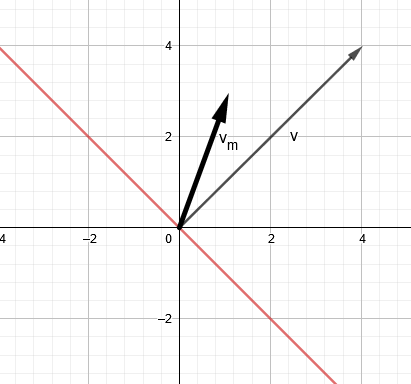
\includegraphics[width=0.5\textwidth]{defpos}
	\caption{$M\vec{v}$ résulte en des vecteurs $\vec v_m$ limités dans la zone située au dessus de la droite}
	\label{fig:mesh1}
\end{figure}

On autorise $\vec v_m$ à être le long de la droite si la matrice est définie semi-positive. Enfin on change de côté si $M$ est définie négative ou semi-négative.\\

Finalement, on raccourcit toute cette définition par le produit scalaire de $\vec v$ et $\vec v_m$. Si le produit scalaire est positif alors les deux vecteurs ne vont pas en contre-sens, il est négatif sinon. Il est nul si l'angle est de 90°, soit les vecteurs de la droite limite. Comme cette définition de ces matrices s'étend aux matrices "symétriques" à coef complexes (les matrices hermitiennes), on a donc un vecteur complexe qu'on dénote généralement $z$.

\[
M_{n \times n} \text{ est définie semi-positive si : } (Mz) \cdot z = z^T M z = \text{produit\textunderscore scalaire}(z, Mz) \geq 0 \quad \text{pour } z \in \mathbb{C}^n
\]

\end{document}
